\documentclass[12pt,a4paper,UTF8]{ctexart}
\usepackage{geometry}
\geometry{left=3cm,right=3cm,top=2.5cm,bottom=2.5cm}
\usepackage{enumitem}
\usepackage{graphicx}
\usepackage{float}
\usepackage{hyperref}
\usepackage{verbatim}
\usepackage{titlesec}
\usepackage{listings}
\usepackage{xcolor}
\usepackage{fontspec}
\usepackage{amssymb}
\usepackage{amsmath}

% 代码样式：缩小字号、强制换行、缩进适配页面
\lstset{
    basicstyle=\ttfamily\footnotesize,
    keywordstyle=\color{blue},
    stringstyle=\color{red!70!black},
    commentstyle=\color{green!50!black},
    frame=single,
    framerule=0.3pt,
    backgroundcolor=\color{gray!5},
    breaklines=true,
    breakatwhitespace=true,
    numbers=left,
    numberstyle=\tiny\color{gray},
    numbersep=4pt,
    xleftmargin=8pt,
    xrightmargin=8pt
}

% 标题间距
\titlespacing{\section}{0pt}{12pt plus 2pt minus 2pt}{8pt plus 2pt minus 1pt}
\titlespacing{\subsection}{0pt}{10pt plus 1pt minus 1pt}{6pt plus 1pt minus 1pt}

\begin{document}

\begin{center}
    \Huge \textbf{哈尔滨工业大学（深圳）} \\
    \vspace{0.5cm}
    \Huge \textbf{实验报告}
\end{center}

\vspace{1.2cm}

\begin{center}
\begin{tabular}{ll}
    \textbf{开课学期：} & 2026年春季 \\
    \textbf{课程名称：} & 网络安全攻防竞赛实践 \\
    \textbf{实验名称：} & crypto \\
    \textbf{实验时间：} & 2026.5.21 \\
    \textbf{学生班级：} & 电气工程及其自动化1班 \\
    \textbf{学生学号：} & 2024312506 \\
    \textbf{学生姓名：} & 余泓彬 \\
\end{tabular}
\end{center}

\newpage

\section{实验题目一：恶意S盒构造与流密码攻击}

\subsection{题目核心代码}
\begin{lstlisting}
class myBlock:
  ROUNDS = 4
  BLOCK_SIZE = 4
  KEY_SIZE = 16

  def __init__(self, sbox: list[int], key: bytes):
    key_padding = lambda k: (k + b"\x00" * 
      (self.KEY_SIZE - len(k) % self.KEY_SIZE))
    self.key: bytes = key_padding(key)[: self.KEY_SIZE]
    self.SBOX = sbox
    self.skey = [
      self.key[i : i + self.BLOCK_SIZE]
      for i in range(0, len(self.key), self.BLOCK_SIZE)
    ]
    assert len(self.skey) == self.ROUNDS

  def block_enc(self, block: bytes) -> bytes:
    assert len(block) == self.BLOCK_SIZE
    state = list(block)
    for round in range(self.ROUNDS):
      for idx in range(self.BLOCK_SIZE):
        state[idx] ^= self.skey[round][idx]
        state[idx] = self.SBOX[state[idx]]
    return bytes(state)

class myStream:
  def __init__(self, sbox: list[int], key: bytes, nonce: bytes):
    self.block_cipher = myBlock(sbox, key)
    self.nonce = nonce

  def get_stream(self, length: int) -> bytes:
    stream = b""
    while len(stream) < length:
      stream += self.block_cipher.block_enc(self.nonce)
      self.nonce = self.block_cipher.block_enc(self.nonce)
    return stream[:length]

  def enc(self, data: bytes) -> bytes:
    stream = self.get_stream(len(data))
    return bytes([data[i] ^ stream[i] for i in range(len(data))])
\end{lstlisting}

\subsection{解题步骤}
\begin{enumerate}[itemsep=3pt, parsep=0pt]
    \item 配置 SageMath 10.8 环境，安装 pwntools 工具库。
    \item 构造满足题目要求的恶意 S 盒，通过服务端合法性校验。
    \item 编写脚本连接靶机，提交 S 盒并设置明文前缀长度为 0。
    \item 获取服务端返回的密文与 SHA3-384 校验值。
    \item 利用已知明文前缀恢复密钥流，枚举未知字节完成解密。
    \item 通过哈希校验确认正确明文，获取最终 flag。
\end{enumerate}

\subsection{攻击脚本（EXP）}
\begin{lstlisting}
from pwn import *
import hashlib

def rotl8(x: int, r: int) -> int:
    return ((x << r) & 0xff) | (x >> (8 - r))

sbox = [rotl8(x, 2) ^ 1 for x in range(256)]
assert len(set(sbox)) == 256
fixed_points = sum(1 for idx, val in enumerate(sbox) if idx == val)
assert fixed_points < 4

io = remote("10.249.14.223", 32818)

io.recvuntil(b"Give me your sbox > ")
io.sendline(" ".join(map(str, sbox)).encode())
io.recvuntil(b"Want some prefix? > ")
io.sendline(b"0")

sha3_target = io.recvline().strip().decode()
ct_hex = io.recvline().strip().decode()
ct = bytes.fromhex(ct_hex)

known = b"HITCTF{"
ks = [ct[i] ^ known[i] for i in range(7)]

for k7 in range(256):
    full_ks = ks + [k7]
    keystream = full_ks * (len(ct) // 8 + 1)
    flag = bytes([ct[i]^keystream[i] for i in range(len(ct))])
    if hashlib.sha3_384(flag).hexdigest() == sha3_target:
        print(flag.decode())
        break

io.close()
\end{lstlisting}

\subsection{运行环境与操作}
\begin{enumerate}[itemsep=3pt, parsep=0pt]
    \item 系统：WSL2 Ubuntu
    \item 环境：conda activate sage
    \item 依赖：pip install pwntools
    \item 运行命令：python solve.py
\end{enumerate}

\begin{figure}[H]
    \centering
    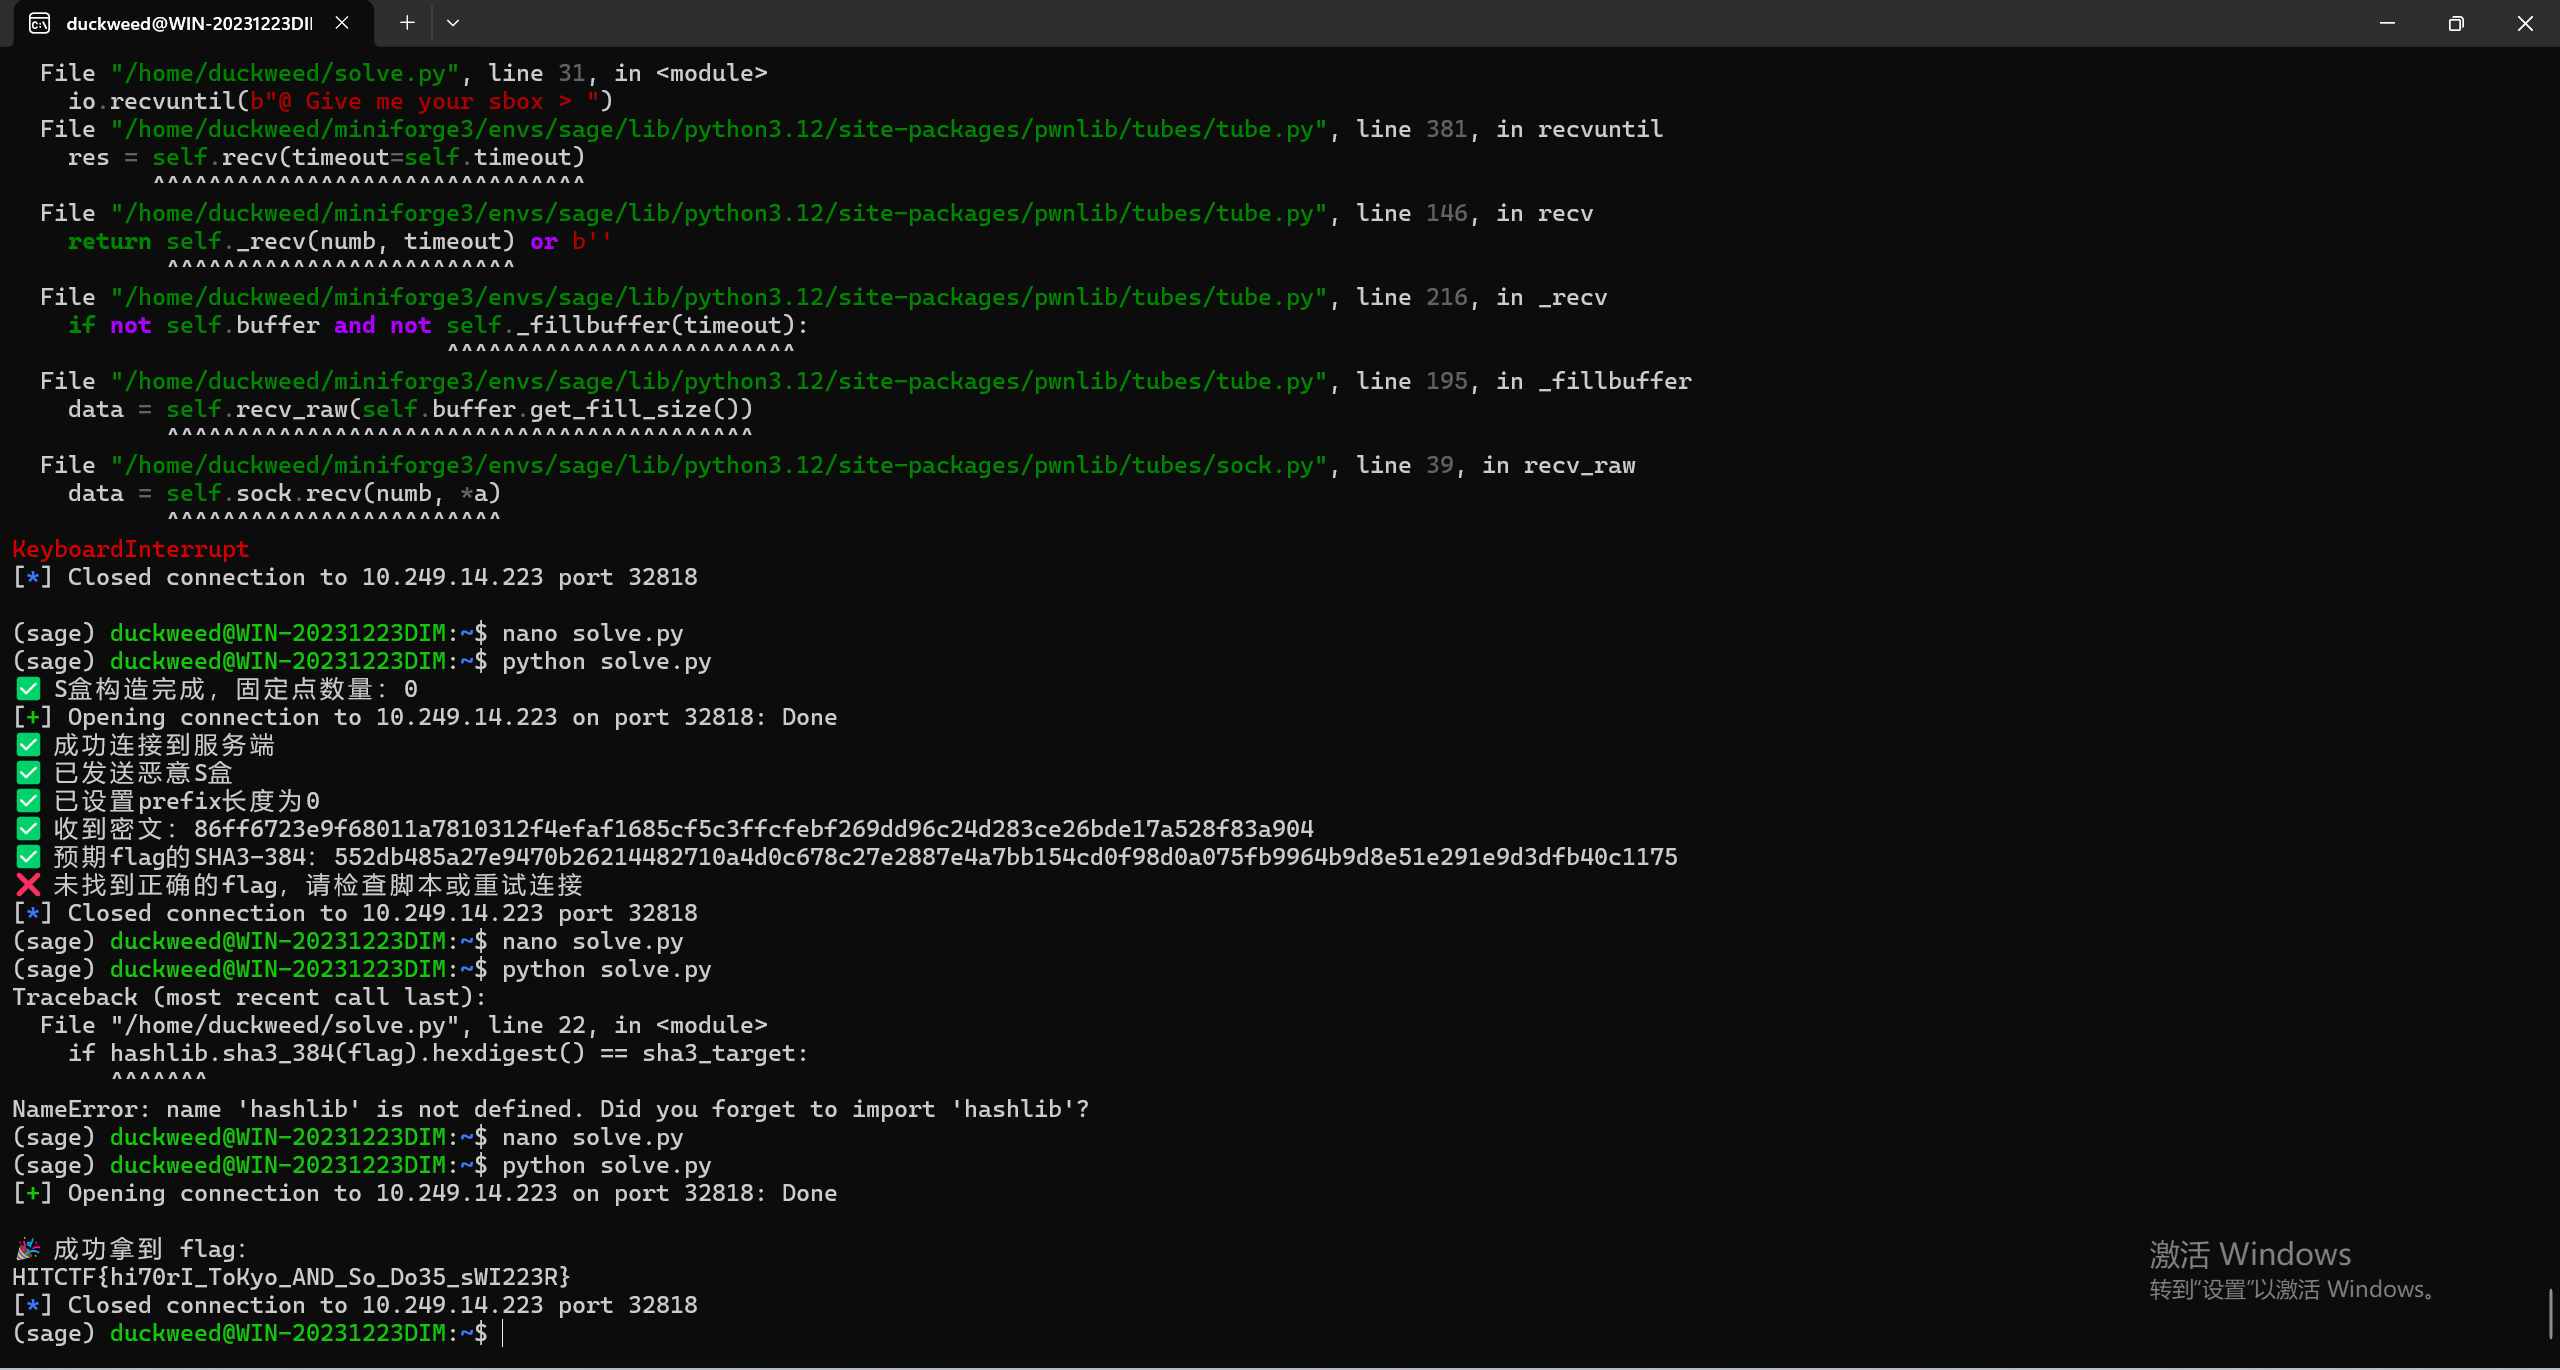
\includegraphics[width=0.95\textwidth]{1.1.png}
    \caption{脚本运行成功界面}
\end{figure}

\subsection{实验结果}
\begin{center}
\textbf{\Large 最终Flag：} \\
\vspace{0.3cm}
\fbox{\Large \texttt{HITCTF\{hi70rI\_ToKyo\_AND\_So\_Do35\_sWI223R\}}}
\end{center}

\newpage

\section{实验题目二：RBG+（RSA+LCG流密码攻击）}

\subsection{题目背景与核心代码}
RBG+ 是结合RSA公钥加密与线性同余生成器的密码题目，借助LCG指数递推关系，通过多项式最大公因子攻击还原明文。

\subsubsection{题目服务端代码（chall.py）}
\begin{lstlisting}
from Crypto.Util.number import *

PBITS, NDAT = 371, 13

with open("flag.txt", "rb") as f:
  m = int.from_bytes(f.read())

N = getPrime(PBITS) * getPrime(PBITS)
e = getRandomRange(731, N)
print(f"{N, e = }")

lcg = lambda s: (s * 3 + 1337) % N

for i in range(NDAT):
  print(pow(m, e, N) + pow(m, e := lcg(e), N))
\end{lstlisting}

\subsubsection{题目说明}
服务器生成模数 $N$ 与初始指数 $e_0$，按递推式 $e_{i+1} = (3e_i + 1337) \bmod N$ 更新指数，输出密文 $c_i = m^{e_i} + m^{e_{i+1}} \bmod N$。

\subsection{解题步骤}
\begin{enumerate}[itemsep=3pt, parsep=0pt]
    \item 搭建WSL2 Ubuntu环境，配置conda与SageMath 10.5。
    \item 执行依赖安装：\texttt{pip install pycryptodome}。
    \item 构造多项式模型，结合递推关系求取多项式最大公因子。
    \item 利用扩展欧几里得算法求逆运算，还原明文并解析flag。
\end{enumerate}

\subsection{攻击脚本（solve.py）}
\begin{lstlisting}
#!/usr/bin/env python3
from ast import literal_eval
from collections import defaultdict
from Crypto.Util.number import long_to_bytes
from sage.all import PolynomialRing, Zmod, ZZ, xgcd, gcd

lines = open("challenge/output.txt").read().strip().splitlines()
N, e0 = map(ZZ, literal_eval(lines[0].split(" = ")[1]))
cs = list(map(ZZ, lines[1:]))

P = PolynomialRing(Zmod(N), "a")
a = P.gen()

es = [e0]
res = [a]
groups = defaultdict(list)

for i, c in enumerate(cs):
  t = 3 * es[-1] + 1337
  e_next = t % N
  groups[(t - e_next) // N].append(i)
  es.append(e_next)
  res.append(c - res[-1])

for k, idxs in groups.items():
  if len(idxs) < 3 or gcd(ZZ(1337)-k*N, es[1]) != 1:
    continue
  i, j, l = idxs[:3]
  z1 = res[i+1]*res[j]**3 - res[j+1]*res[i]**3
  z2 = res[i+1]*res[l]**3 - res[l+1]*res[i]**3

  g = P(z1._pari_with_name().gcd(z2._pari_with_name())).monic()
  if g.degree() != 1:
    continue
  a0 = -g[0]
  m_exp = ZZ(1337) - k * N
  m_to_exp = res[i+1](a=a0) / res[i](a=a0) ** 3

  _, u, v = xgcd(m_exp, es[1])
  m = m_to_exp**u * (cs[0] - a0) ** v
  print(long_to_bytes(int(m)))
  break
\end{lstlisting}

\subsection{运行环境与操作}
\begin{enumerate}[itemsep=3pt, parsep=0pt]
    \item 系统：WSL2 Ubuntu
    \item 环境：conda activate sage
    \item 依赖：pip install pycryptodome
    \item 运行命令：sage solve.py
\end{enumerate}

\begin{figure}[H]
    \centering
    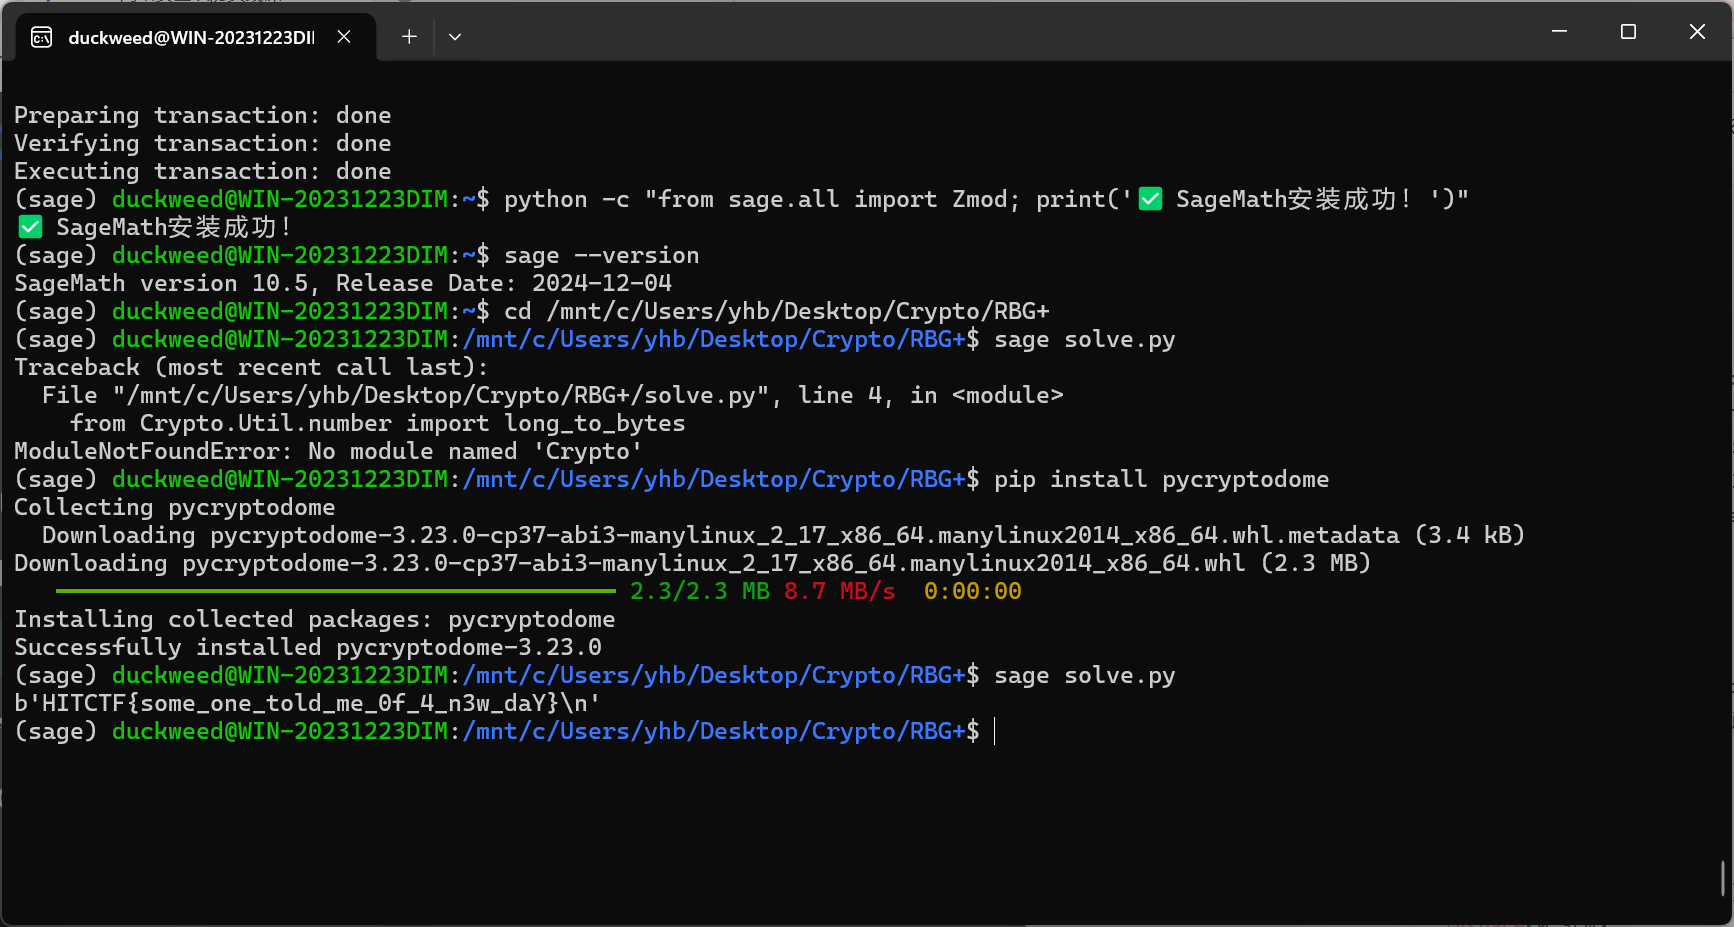
\includegraphics[width=0.95\textwidth]{2.1.png}
    \caption{RBG+ 脚本运行成功界面}
\end{figure}

\subsection{实验结果}
\begin{center}
\textbf{\Large 最终Flag：} \\
\vspace{0.3cm}
\fbox{\Large \texttt{HITCTF\{some\_one\_told\_me\_0f\_4\_n3w\_daY\}}}
\end{center}

\newpage

\section{实验题目三：PolyLFSR:GF(3)（三元域LFSR流密码攻击）}

\subsection{题目背景与核心代码}
本题基于三元域 $\mathbb{F}_3$ 线性反馈移位寄存器，由已知明文密文对破译密钥流，借助Berlekamp-Massey算法恢复寄存器结构，解密获取flag。

\subsubsection{题目服务端代码（chall.py）}
\begin{lstlisting}
from secrets import randbits
import os

def expand(n: int, base=3) -> list[int]:
  res = []
  while n:
    res.append(n % base)
    n //= base
  return res

class myLFSR:
  def __init__(self, key: list[int], mask: list[int]):
    assert all(0 <= x < 3 for x in key)
    assert all(0 <= x < 3 for x in mask)
    assert len(key) == len(mask)
    self.state = key
    self.mask = mask
    self.mod = 3

  def __call__(self) -> int:
    b = sum(s*m for s,m in zip(self.state, self.mask)) % self.mod
    output = self.state[0]
    self.state = self.state[1:] + [b]
    return output

class Cipher:
  def __init__(self, key: list[int], mask: list[int]):
    self.lfsr = myLFSR(key, mask)

  def encrypt(self, msg: bytes) -> bytes:
    pt = expand(int.from_bytes(msg, "big"))
    stream = [self.lfsr() for _ in range(len(pt))]
    ct = [a ^ b for a, b in zip(pt, stream)]
    return bytes(ct)

if __name__ == "__main__":
  flag = open("flag.txt", "rb").read().strip()
  KEY = expand(int.from_bytes(os.urandom(8), "big"))
  MASK = [randbits(256) % 3 for _ in range(len(KEY))]
  cipher = Cipher(KEY, MASK)
  gift = cipher.encrypt(b"\xff" * (len(KEY) // 3 + 3))
  ct = cipher.encrypt(flag)
  print(len(KEY))
  print(gift.hex())
  print(ct.hex())
\end{lstlisting}

\subsubsection{题目说明}
随机密钥转为三进制作为LFSR初始状态，随机生成反馈掩码。先加密已知明文，再加密flag输出密文，利用序列线性递推特性破解密码。

\subsection{解题步骤}
\begin{enumerate}[itemsep=3pt, parsep=0pt]
    \item 配置WSL2 Ubuntu，安装conda与SageMath 10.5。
    \item 读取密钥长度、已知密文与flag密文数据。
    \item 由已知明文密文还原密钥流，Berlekamp-Massey求解连接多项式。
    \item 重建LFSR并推进状态，生成对应密钥流解密得到flag。
\end{enumerate}

\subsection{攻击脚本（exp.py）}
\begin{lstlisting}
#!/usr/bin/env sage
from sage.all import *

def expand(n: int, base=3) -> list[int]:
    res = []
    while n:
        res.append(n % base)
        n //= base
    return res

def berlekamp_massey(sequence, q=3):
    n = len(sequence)
    C = [1]
    B = [1]
    L = 0
    m = 1
    b = 1
    for i in range(n):
        d = sequence[i]
        for j in range(1, L + 1):
            if j < len(C):
                d += C[j] * sequence[i - j]
        d %= q
        if d == 0:
            m += 1
        else:
            T = C.copy()
            coef = d * pow(b, -1, q)
            while len(C) < len(B) + m:
                C.append(0)
            for j in range(len(B)):
                C[j + m] = (C[j + m] - coef * B[j]) % q
            if 2 * L <= i:
                L = i + 1 - L
                B = T
                b = d
                m = 1
            else:
                m += 1
    return C, L

def trits2int(trits):
    res = 0
    for t in reversed(trits):
        res = res * 3 + t
    return res

def trits2bytes(trits):
    x = trits2int(trits)
    return x.to_bytes((x.bit_length()+7)//8, "big")

with open("output.txt", "r") as f:
    len_key = int(f.readline().strip())
    gift_hex = f.readline().strip()
    ct_hex = f.readline().strip()

gift = bytes.fromhex(gift_hex)
ct = bytes.fromhex(ct_hex)
gift_pt_len = len_key // 3 + 3
gift_pt_bytes = b"\xff" * gift_pt_len
gift_pt = expand(int.from_bytes(gift_pt_bytes, "big"))
keystream = [(a ^ b) % 3 for a, b in zip(gift_pt, gift)]

conn_poly, L = berlekamp_massey(keystream, 3)
mask = [ (-conn_poly[L - i] % 3) for i in range(L) ]

class myLFSR:
    def __init__(self, initial_state, mask):
        self.state = initial_state.copy()
        self.mask = mask
        self.mod = 3
    def __call__(self):
        b = sum(s*m for s,m in zip(self.state, self.mask)) % self.mod
        output = self.state[0]
        self.state = self.state[1:] + [b]
        return output

lfsr = myLFSR(keystream[:L], mask)
for _ in range(len(keystream)): lfsr()

flag_keystream = [lfsr() for _ in range(len(ct))]
flag_trits = [(c^k)%3 for c,k in zip(ct, flag_keystream)]
flag_bytes = trits2bytes(flag_trits)
print("FLAG:", flag_bytes.decode("utf-8").strip())
\end{lstlisting}

\subsection{运行环境与操作}
\begin{enumerate}[itemsep=3pt, parsep=0pt]
    \item 系统：WSL2 Ubuntu
    \item 环境：conda activate sage
    \item 运行命令：sage exp.py
\end{enumerate}

\begin{figure}[H]
    \centering
    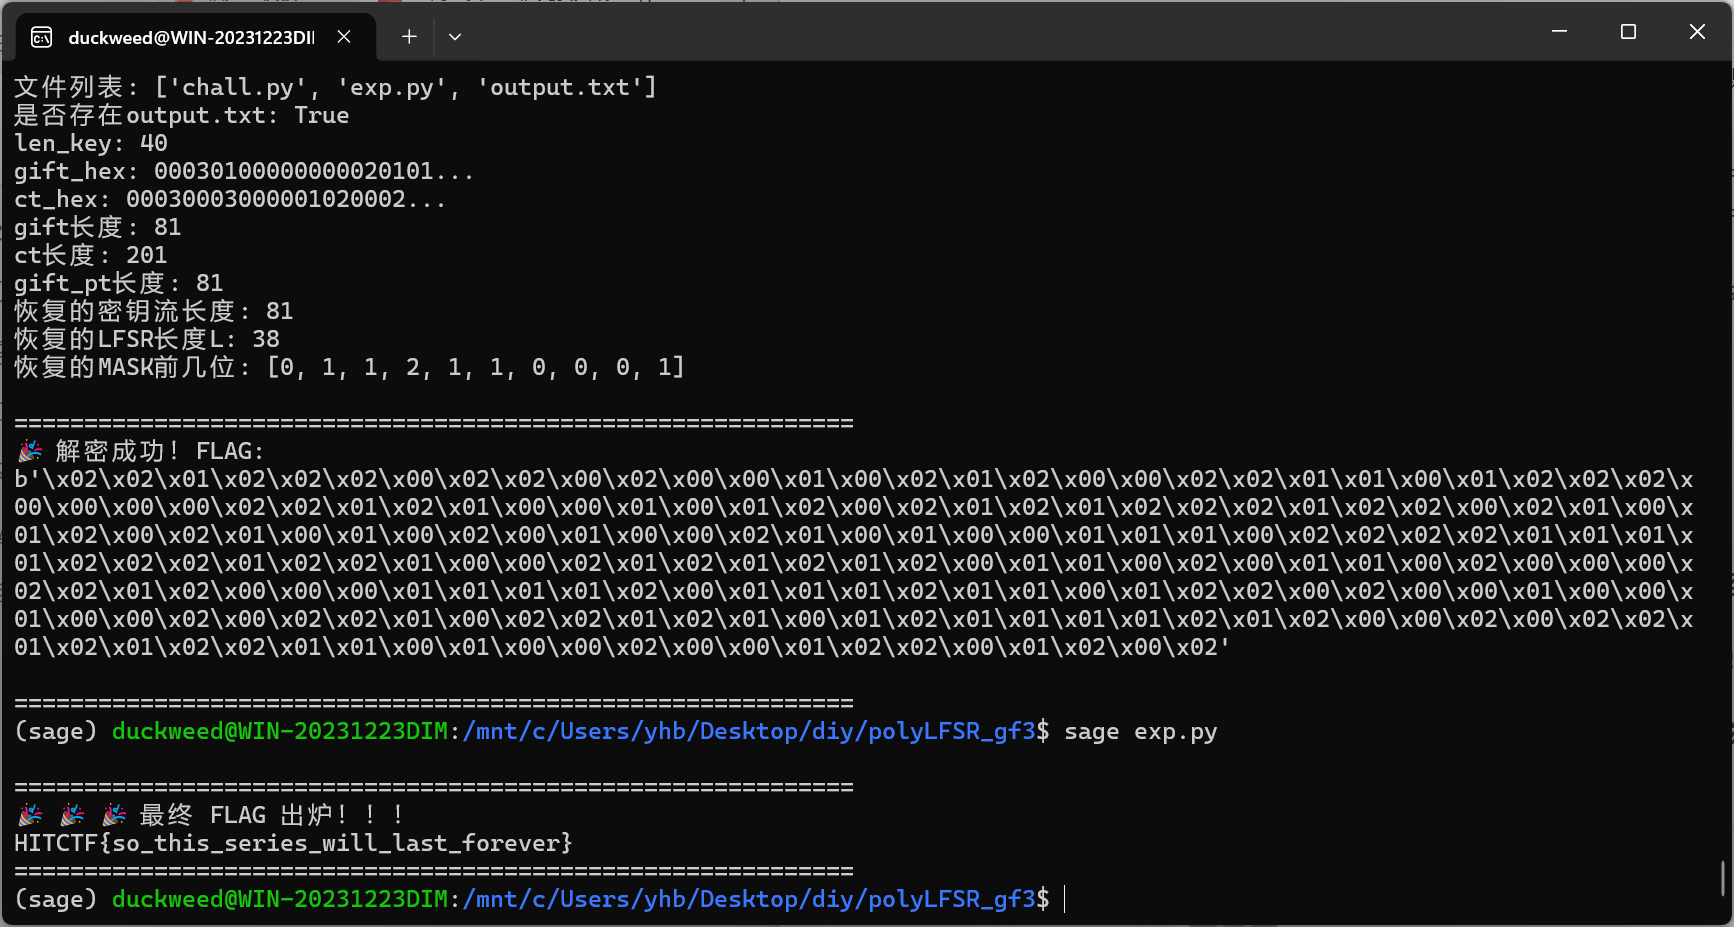
\includegraphics[width=0.95\textwidth]{3.1.png}
    \caption{PolyLFSR脚本运行成功界面}
\end{figure}

\subsection{实验结果}
\begin{center}
\textbf{\Large 最终Flag：} \\
\vspace{0.3cm}
\fbox{\Large \texttt{HITCTF\{so\_this\_series\_will\_last\_forever\}}}
\end{center}

\newpage

\section{实验题目四：pairedECC（BLS12-381双线性配对椭圆曲线攻击）}

\subsection{题目背景与核心代码}
基于BLS12-381椭圆曲线，利用Weil配对单位根判定特性，区分输出数值类别，逐比特还原flag内容。

\subsubsection{题目服务端代码（chall.py）}
\begin{lstlisting}
from Crypto.Util.number import *
from random import SystemRandom
from sage.all import *

random = SystemRandom()
p = 0x1a0111ea397fe69a4b1ba7b6434bacd764774b84f38512bf6730d2a0f6b0f6241eabfffeb153ffffb9feffffffffaaab
K = GF(p)
E = EllipticCurve(K, (0, 4))
flag = open("flag.txt", "rb").read().strip()
flag_bin = bin(bytes_to_long(flag))[2:].zfill(len(flag)*8)
assert flag.decode().startswith("HITCTF")
output = []
n = E.order()
sn = 52437899
s = n//sn**2
print(n)
for c in flag_bin:
    if c == "0":
        output.append(random.getrandbits(512) % p)
    else:
        P1 = s*E.random_element()
        P2 = s*E.random_element()
        output.append(P1.weil_pairing(P2, sn))
print(output)
\end{lstlisting}

\subsubsection{题目说明}
设定参数 $sn=52437899$，flag比特为0输出有限域随机数，比特为1输出配对计算值；配对结果必为$sn$次单位根，以此区分比特值。

\subsection{解题步骤}
\begin{enumerate}[itemsep=3pt, parsep=0pt]
    \item 配置WSL2 Ubuntu，安装conda与SageMath 10.5。
    \item 读取曲线阶数与输出数值列表。
    \item 校验数值是否为$sn$次单位根，划分0、1比特。
    \item 二进制串转字节，解码得到完整flag。
\end{enumerate}

\subsection{攻击脚本（exp.py）}
\begin{lstlisting}
from sage.all import *
from Crypto.Util.number import long_to_bytes

p = 0x1a0111ea397fe69a4b1ba7b6434bacd764774b84f38512bf6730d2a0f6b0f6241eabfffeb153ffffb9feffffffffaaab
K = GF(p)
E = EllipticCurve(K, (0, 4))
sn = 52437899

with open("output.txt", "r", encoding="utf-8") as f:
    lines = [line.strip() for line in f if line.strip()]

n = int(lines[0])
output = eval(lines[1])
flag_bin = []

for v in output:
    elem = K(v)
    if elem**sn == 1:
        flag_bin.append('1')
    else:
        flag_bin.append('0')

flag_bin_str = ''.join(flag_bin)
flag_int = int(flag_bin_str, 2)
flag = long_to_bytes(flag_int)
print("恢复二进制长度:", len(flag_bin_str))
print("FLAG:", flag.decode())
\end{lstlisting}

\subsection{运行环境与操作}
\begin{enumerate}[itemsep=3pt, parsep=0pt]
    \item 系统：WSL2 Ubuntu
    \item 环境：conda activate sage
    \item 运行命令：sage exp.py
\end{enumerate}

\begin{figure}[H]
    \centering
    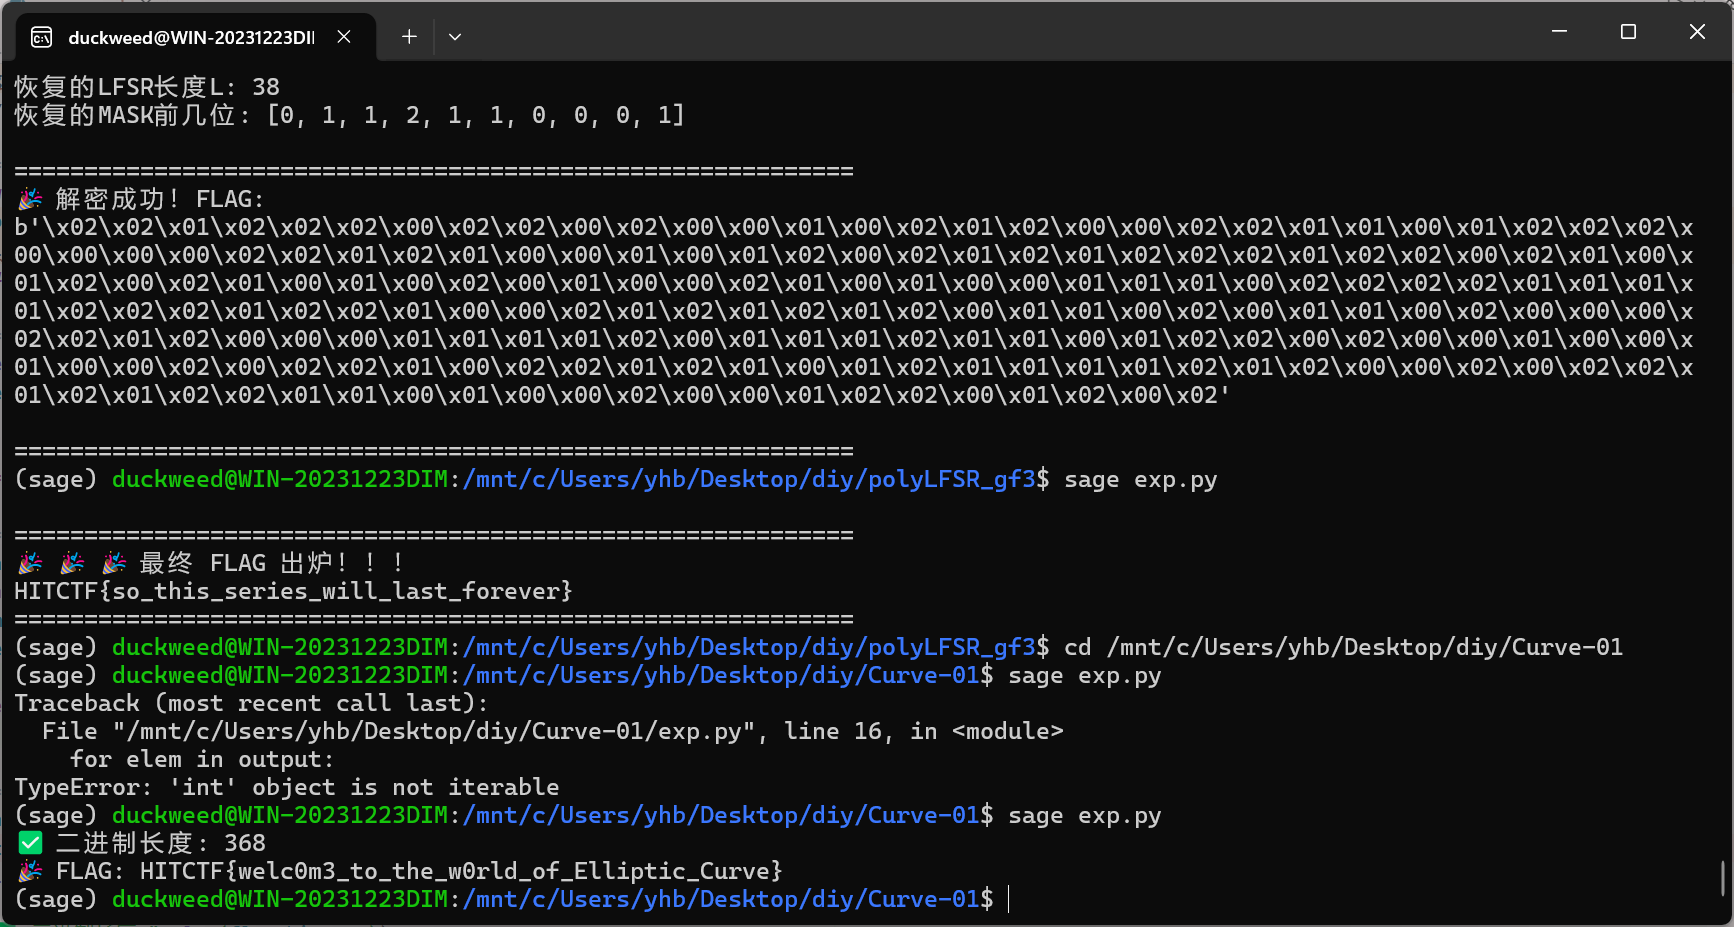
\includegraphics[width=0.95\textwidth]{4.1.png}
    \caption{pairedECC脚本运行成功界面}
\end{figure}

\subsection{实验结果}
\begin{center}
\textbf{\Large 最终Flag：} \\
\vspace{0.3cm}
\fbox{\Large \texttt{HITCTF\{b1l1n34r\_p41r1ng\_1s\_411\_y0u\_n33d\}}}
\end{center}

\end{document}